\documentclass[a4paper, 11pt]{article}

\usepackage[utf8]{inputenc}
\usepackage[T1]{fontenc}
\usepackage[francais]{babel} 
\usepackage{amsmath} % pour les formules de maths
\usepackage{amssymb} % pour des symboles
\usepackage{mathrsfs} % pour avoir acces a des jolies lettres calligrafiées. :)
\usepackage{listings} % pour le code source
\usepackage{color} % pour les couleurs
\usepackage{graphicx} % pour les graphiques (images)
\usepackage{fancyhdr} % pour utiliser le pagestyle fancy
\usepackage[headheight=14pt]{geometry} % pour les marges

\geometry{hmargin=3cm}

\title{Methods and Heuristics for Learning and Optimization}
\author{Romain Mencattini}
\date{\today}

\pagestyle{fancy} % pour avoir des entetes et des pieds de page
\renewcommand\headrulewidth{0.6pt}
\fancyhead[L]{Romain Mencattini} % haut de page gauche
\fancyhead[R]{Université de Genève \today} % haut de page droite

\begin{document}
\maketitle
\newpage
\tableofcontents
\newpage

\section{Le voyageur de commerce}
Il s'agit du problème sur lequel nous allons tester l'algorithme du recuit simulé.\\
Détaillons le de manière mathématique.\\
Nous avons un ensemble de villes : $V$. Où $v = \{x,y\} \in V$. est une ville qui avec une coordonnée $x$ et une coordonnée $y$ qui appratiennent 
à $\mathbb{N}$.

On veut visiter toutes les villes, une et une seule fois. Notre résultat sera une permutation de ces villes: $[v_1,v_2,...,v_N]$.
Une liste avec $N$ villes. Où $v_1$ 
sera la première ville visitée, $v_2$ la deuxième etc.

On utilise la distance euclidienne :
\begin{center}
\begin{math}
 euclidienne(v_1,v_2) = \sqrt{(v_{1_x} - v_{2_x})^2 + (v_{1_y} - v_{2_y})^2}
\end{math} 
\end{center}

On veut minimiser la distance totale qui est:
\begin{center}
 \begin{math}
  d_{total} = \sum\limits_{i=2}^{N} euclidienne(v_{i-1},v_i)
 \end{math}
\end{center}



\section{Algorithme}
Pour ce faire on va comparer plusieurs algorithmes.

\subsection{Recuit simulé}
Voici le principe de l'algorithme du recuit simulé, ou SA.
\begin{enumerate}
 \item Choisir une solution initiale, $s_0$, qui est une permutation des villes.
 \item Calculer la température initiale. Pour ce faire, on fait 100 transformations élémentaires aléatoires, et on regarde le $\Delta$ d'énergie. En 
 résolvant l'équation:
 \begin{center}
  \begin{math}
   e^{\frac{-<\Delta E>}{T_0}} = 0.5
  \end{math}
 \end{center}
 
 \item Effectuer une transformation élémentaire aléatoire pour obtenir $s_1$.
 \item On applique la règle d'acceptation (de Métropolis):
 \begin{center}
  \begin{displaymath}
    P = 
    \left\lbrace
      \begin{array}{ll}
	1 & \text{si } \Delta E < 0 \\
	e^{\frac{-\Delta E}{T}} & \text{sinon } \\
      \end{array}
    \right.
\end{displaymath}
 \end{center}
 On accepte si $rand() < P$ où $rand() \in [0,1[$.
 Si on accepte $s_0 = s_1$.

 \item On considère qu'un équilibre est atteint lorsqu'on a accepté $12n$ changements ou qu'il y a eu $100n$ perturbations sans 
 changements.
 
 \item Lorsqu'on est en équilibre, on diminue la température: $T_{k+1} = 0.9 T_k$.
 
 \item On arrête l'algorithme lorsqu'on a diminué trois fois la température, sans qu'il y ait eu aucun changements de solutions. On 
 considèrera que la solution est suffisemment stable pour qu'elle ne change plus.

\end{enumerate}

Il reste à expliquer ce que signifie une perturbation élémentaire. Cela consiste en une nouvelle permutation où on aura échangé deux 
villes.

\subsection{Greedy}
L'algorithme est plus simple que celui du recuit.
Il faut:
\begin{enumerate}
 \item Choisir une ville aléatoire, $v_0$.
 \item Ajouter la ville la plus prochaine à notre solution.
 \item Répéter l'étape 2. jusqu'à ce qu'on ait vue toutes les viles.
\end{enumerate}

Suivant le choix du développeur, on peut choisir d'ajouter la première ville, à la fin pour avoir une boucle.
Cet algorithme est totalement déterministe pour un $V$ fixé et une ville initiale $v_0$ fixée.

\section{Mesures et Résultats}
Voici les résultats obtenus en moyenne lors de dix lancés.

\subsection{Cities.dat}
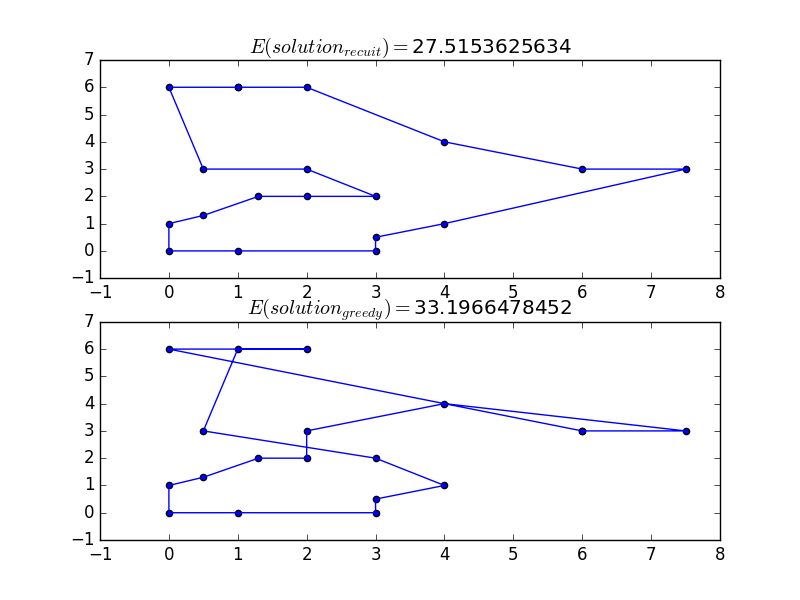
\includegraphics[scale=0.75]{best}
On remarque que les deux solutions sont assez bonnes, (visuellement et en terme d'énergie). On peut noter que le recuit est meilleur dans 
ce cas.
Il s'agit d'un seul lancé pour illustré, ce à quoi ça ressemble. Voici le tableau avec la moyenne:\\
\begin{tabular}{|l | c |c |}
\hline
Cities.dat & & \\
\hline
  & Moyenne & Déviation standard\\
 \hline
Greedy & 33.2325687408	& 1.77688\\
\hline
Recuit & 31.3042554855	 & 1.71704\\
\hline
\end{tabular}

\paragraph{}On voit que le recuit est en moyenne meilleur. Il n'a que peu de déviation standard. Environ 3\% de la valeur moyenne d'énergie.
Les deux algorithmes sont donc assez stable.	

Les résultats moyens sont un peu éloigné du meilleur résultat trouvé plus haut. Il y a moins de 10\% de différence, ce qui signifie qu'on
trouve de bon solution, assez proche de l'optimum global.

\subsection{Cities2.dat}
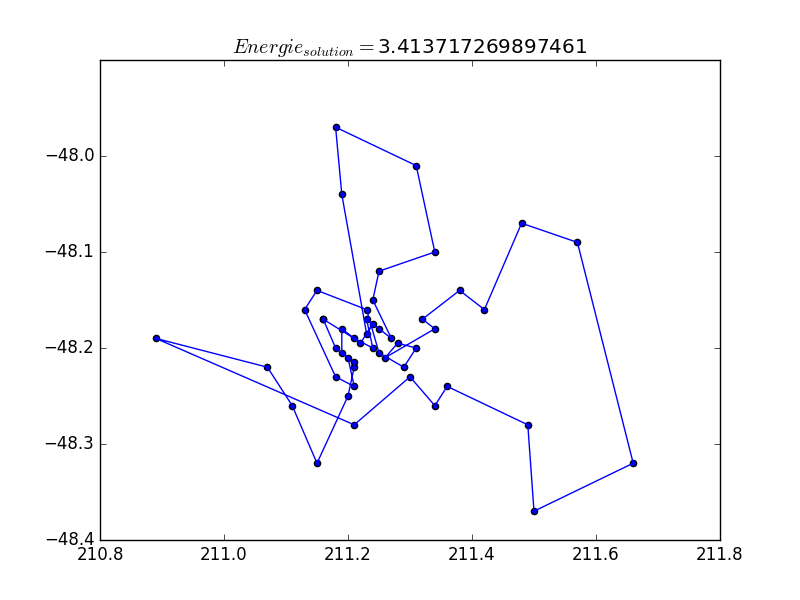
\includegraphics[scale=0.75]{cities2}
Les points centraux étant très proches, cela peut engendré beaucoup de différences d'un lancé à un autre. Il est également plus compliqué
de trouver l'optimum.

Voici le tableau avec la moyenne:\\
\begin{tabular}{|l | c |c |}
\hline
Cities2.dat & & \\
\hline
  & Moyenne & Déviation standard\\
 \hline
Greedy & 3.46352212408	& 0.166237\\
\hline
Recuit & 3.54229936614	 & 0.171651\\
\hline
\end{tabular}

\paragraph{}
Le point positif est que la déviation standard est très faible. On a confirmation
que les algorithmes sont stables sur plusieurs lancés.

Cette fois ci, le \textit{greedy} est légèrement meilleur. Nous pensons que cela vient
des points centraux très proches qui peuvent perturber l'algorithme du recit  et engendré des
résultats moins bon.

\subsection{CitiesN.dat}
Pour les versions avec $n=\{50,60,80,100\}$, nous avons généré des points en cercle, afin de savoir
le résultat optimal et visualiser à quel point nos algorithmes trouvent la solution optimale.

L'algorithme \textit{greedy} trouve toujours l'optimum global, car en prenant le point le plus proche
dans un cercle, on trouve la meilleure solution. Ce n'est donc pertinant que pour nous donner la valeur optimal comme comparaison.

\subsubsection{Cities50.dat}
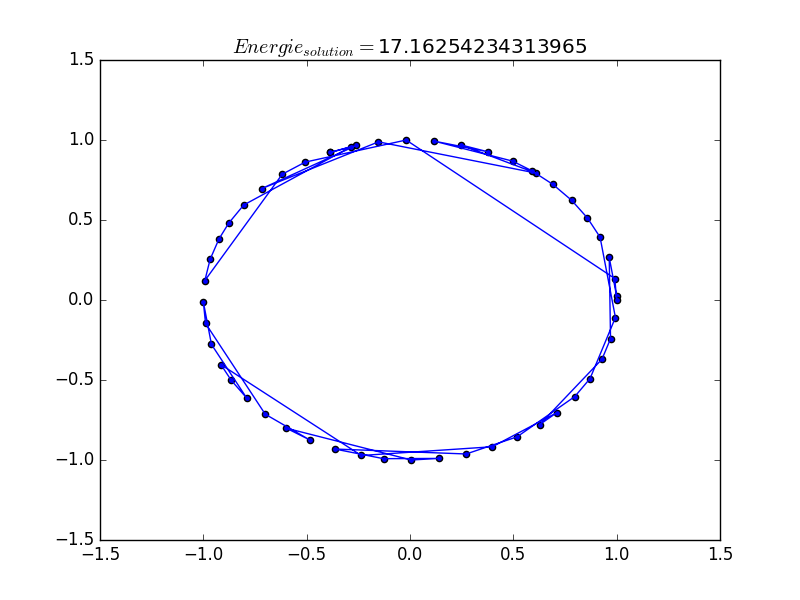
\includegraphics[scale=0.75]{cities50}

Voici le tableau avec la moyenne:\\
\begin{tabular}{|l | c |c |}
\hline
Cities50.dat & & \\
\hline
  & Moyenne & Déviation standard\\
  \hline
Greedy & 6.27877907753	 & 1.50789e-07 \\
\hline
Recuit & 16.9541293144	 & 1.70877\\
\hline
\end{tabular}

\subsubsection{Cities60.dat}
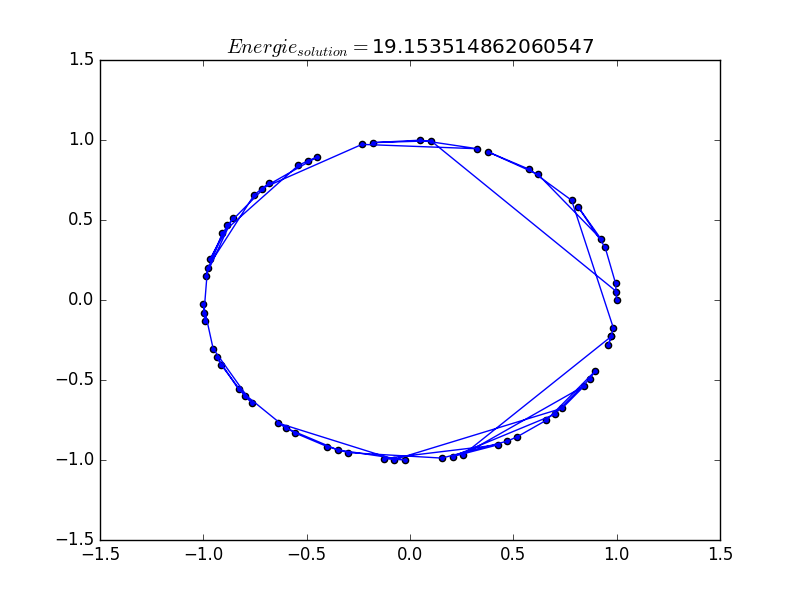
\includegraphics[scale=0.75]{cities60}

Voici le tableau avec la moyenne:\\
\begin{tabular}{|l | c |c |}
\hline
Cities60.dat & & \\
\hline
  & Moyenne & Déviation standard\\
  \hline
Greedy & 6.31829538345	 & 0.051879\\
\hline
Recuit & 19.7690262794	 & 2.64644\\
\hline
\end{tabular}

\subsubsection{Cities80.dat}
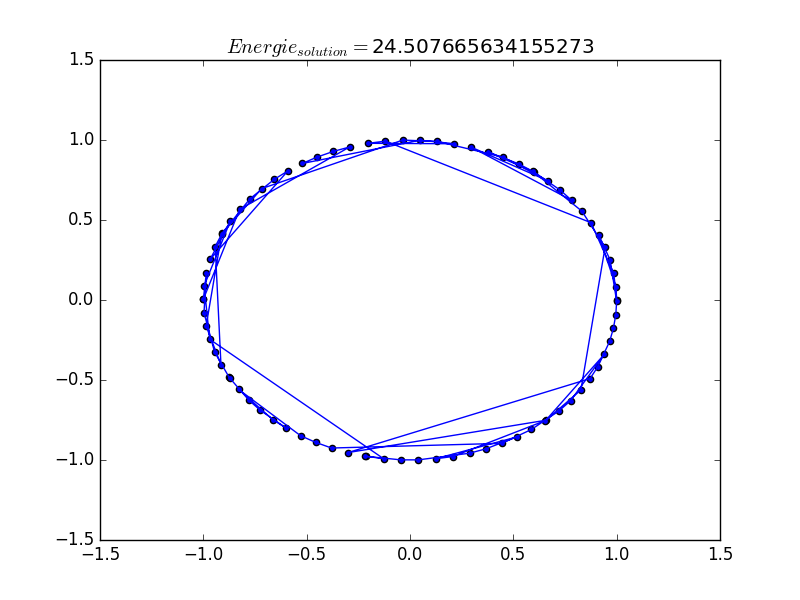
\includegraphics[scale=0.75]{cities80}

Voici le tableau avec la moyenne:\\
\begin{tabular}{|l | c |c |}
\hline
Cities80.dat & & \\
\hline
  & Moyenne & Déviation standard\\
  \hline
Greedy & 6.28134675026	 & 5.43678e-07\\
\hline
Recuit & 27.2583179474	 & 2.54419\\
\hline
\end{tabular}

\subsubsection{Cities100.dat}
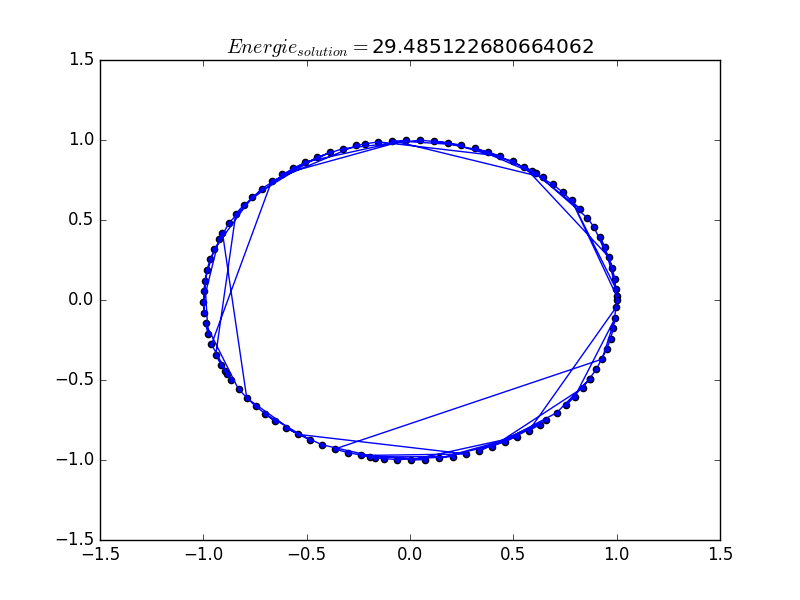
\includegraphics[scale=0.75]{cities100}

Voici le tableau avec la moyenne:\\
\begin{tabular}{|l | c |c |}
\hline
Cities100.dat & & \\
\hline
  & Moyenne & Déviation standard\\
  \hline
Greedy & 6.28206834793	& 3.69356e-07\\
\hline
Recuit & 31.6346078873	 & 2.16477\\
\hline
\end{tabular}

\subsubsection{Remarques}
On voit que la valeur de l'algorithme \textit{greedy} tend vers $d\pi$ où $d=2$. On tend donc bien vers le perimètre d'un cercle comme 
valeur optimale.
Concernant le recuit, on remarque que la majorité de la solution est bien placée, sauf certains points (environ 10\% de $n$), ce qui
fait augmenter l'énergie.

On peut imaginer que le paysage étant très irrégulier cela influencer le résultat. Il est également possible que les valeurs des 
paramètres d'acceptations peuvent jouer. Ou bien la manière de diminuer la température.

\end{document}